\documentclass{beamer}
\usepackage{appendixnumberbeamer}

\mode<presentation>{\usetheme[subsectionpage=progressbar,block=fill,numbering=none]{metropolis}}

\usepackage[sfdefault]{FiraSans} %% option 'sfdefault' activates Fira Sans as the default text font
\usepackage[english]{babel}
% \usepackage[utf8]{inputenc}

\usepackage{graphicx} % Allows including images
\usepackage{pgfplots}
\usepackage{caption}
\usepackage{booktabs} % Allows the use of \toprule, \midrule and \bottomrule in tables
\usepackage{multicol}

% Math packages
\usepackage{amsmath}
\usepackage{mathtools}
\usepackage{amssymb}
\usepackage{mathpartir}
\usepackage{stmaryrd}
\usepackage{centernot}
\usepackage[normalem]{ulem}

%% Coding
\usepackage[outputdir=build]{minted}

% Coloured boxes
\usepackage{tcolorbox}
\colorlet{alert}{mLightBrown}
\colorlet{mLightBrownTransparent}{white!70!mLightBrown}
\newtcolorbox{alertbox}
{standard jigsaw, opacityback=0,colframe=alert}
\newtcolorbox{tbox}
{standard jigsaw, opacityback=0,opacityframe=0}

\newcommand{\haskell}[1]{\mintinline{haskell}{#1}}

\title{Engaging, Large-Scale Functional Programming Education in Physical and Virtual Space} % the title on the title page

\author{Kevin Kappelmann, Jonas Rädle, Lukas Stevens} % Your name
\institute[TU Munich]{Technical University of Munich}
\date{March 16, 2022} % Date, can be changed to a custom date

\begin{document}

\maketitle

%------------------------------------------------
\section{Challenges}
% Soaring Enrolments
\begin{frame}{Soaring Enrolments}
\only<1>{\centerline{\Large{\alert{1. Number of Computer Science students exploded}}}}
\only<2->{\centerline{Example: Computer Science at TU Munich}

\pause
\begin{multicols}{2}
\begin{figure}
\centering
\captionsetup{justification=centering}
% somehow this needs to be 1.02 when it is 1 below
\resizebox{1.03\linewidth}{!}{
\begin{tikzpicture}
\begin{axis}[
    ymin=0,
    x tick label style={/pgf/number format/.cd,%
      set thousands separator={}}
  ]
  \addplot +[color=red, mark options={fill=red}] coordinates {
    (2013, 3555)
    (2014, 3815)
    (2015, 4240)
    (2016, 4744)
    (2017, 5399)
    (2018, 5986)
    (2019, 6458)
    (2020, 7444)
    (2021, 8253)
  };
\end{axis}
\end{tikzpicture}
}
\caption*{Number of CS students\\(132\% increase)}
\end{figure}

\columnbreak

\begin{figure}
\centering
\captionsetup{justification=centering}
\resizebox{\linewidth}{!}{
\begin{tikzpicture}
\begin{axis}[
    ymin=0,
    x tick label style={/pgf/number format/.cd,%
      set thousands separator={}}
  ]
  \addplot coordinates {
    (2013, 439)
    (2014, 449)
    (2015, 432)
    (2016, 436)
    (2017, 438)
    (2018, 450)
    (2019, 500)
    (2020, 529)
    (2021, 573)
  };
\end{axis}
\end{tikzpicture}
}
\caption*{Number of CS academic staff (31\% increase)}
\end{figure}
\end{multicols}
}
\visible<3>{\centerline{\Large{\alert{1000+ students per course are the new normal}}}}
\end{frame}

\begin{frame}{The Pandemic}
\only<1>{\centerline{\Large{\alert{2. Radical transition to online classes}}}}
\only<2>{\centerline{How can we go from here\dots}
\begin{figure}
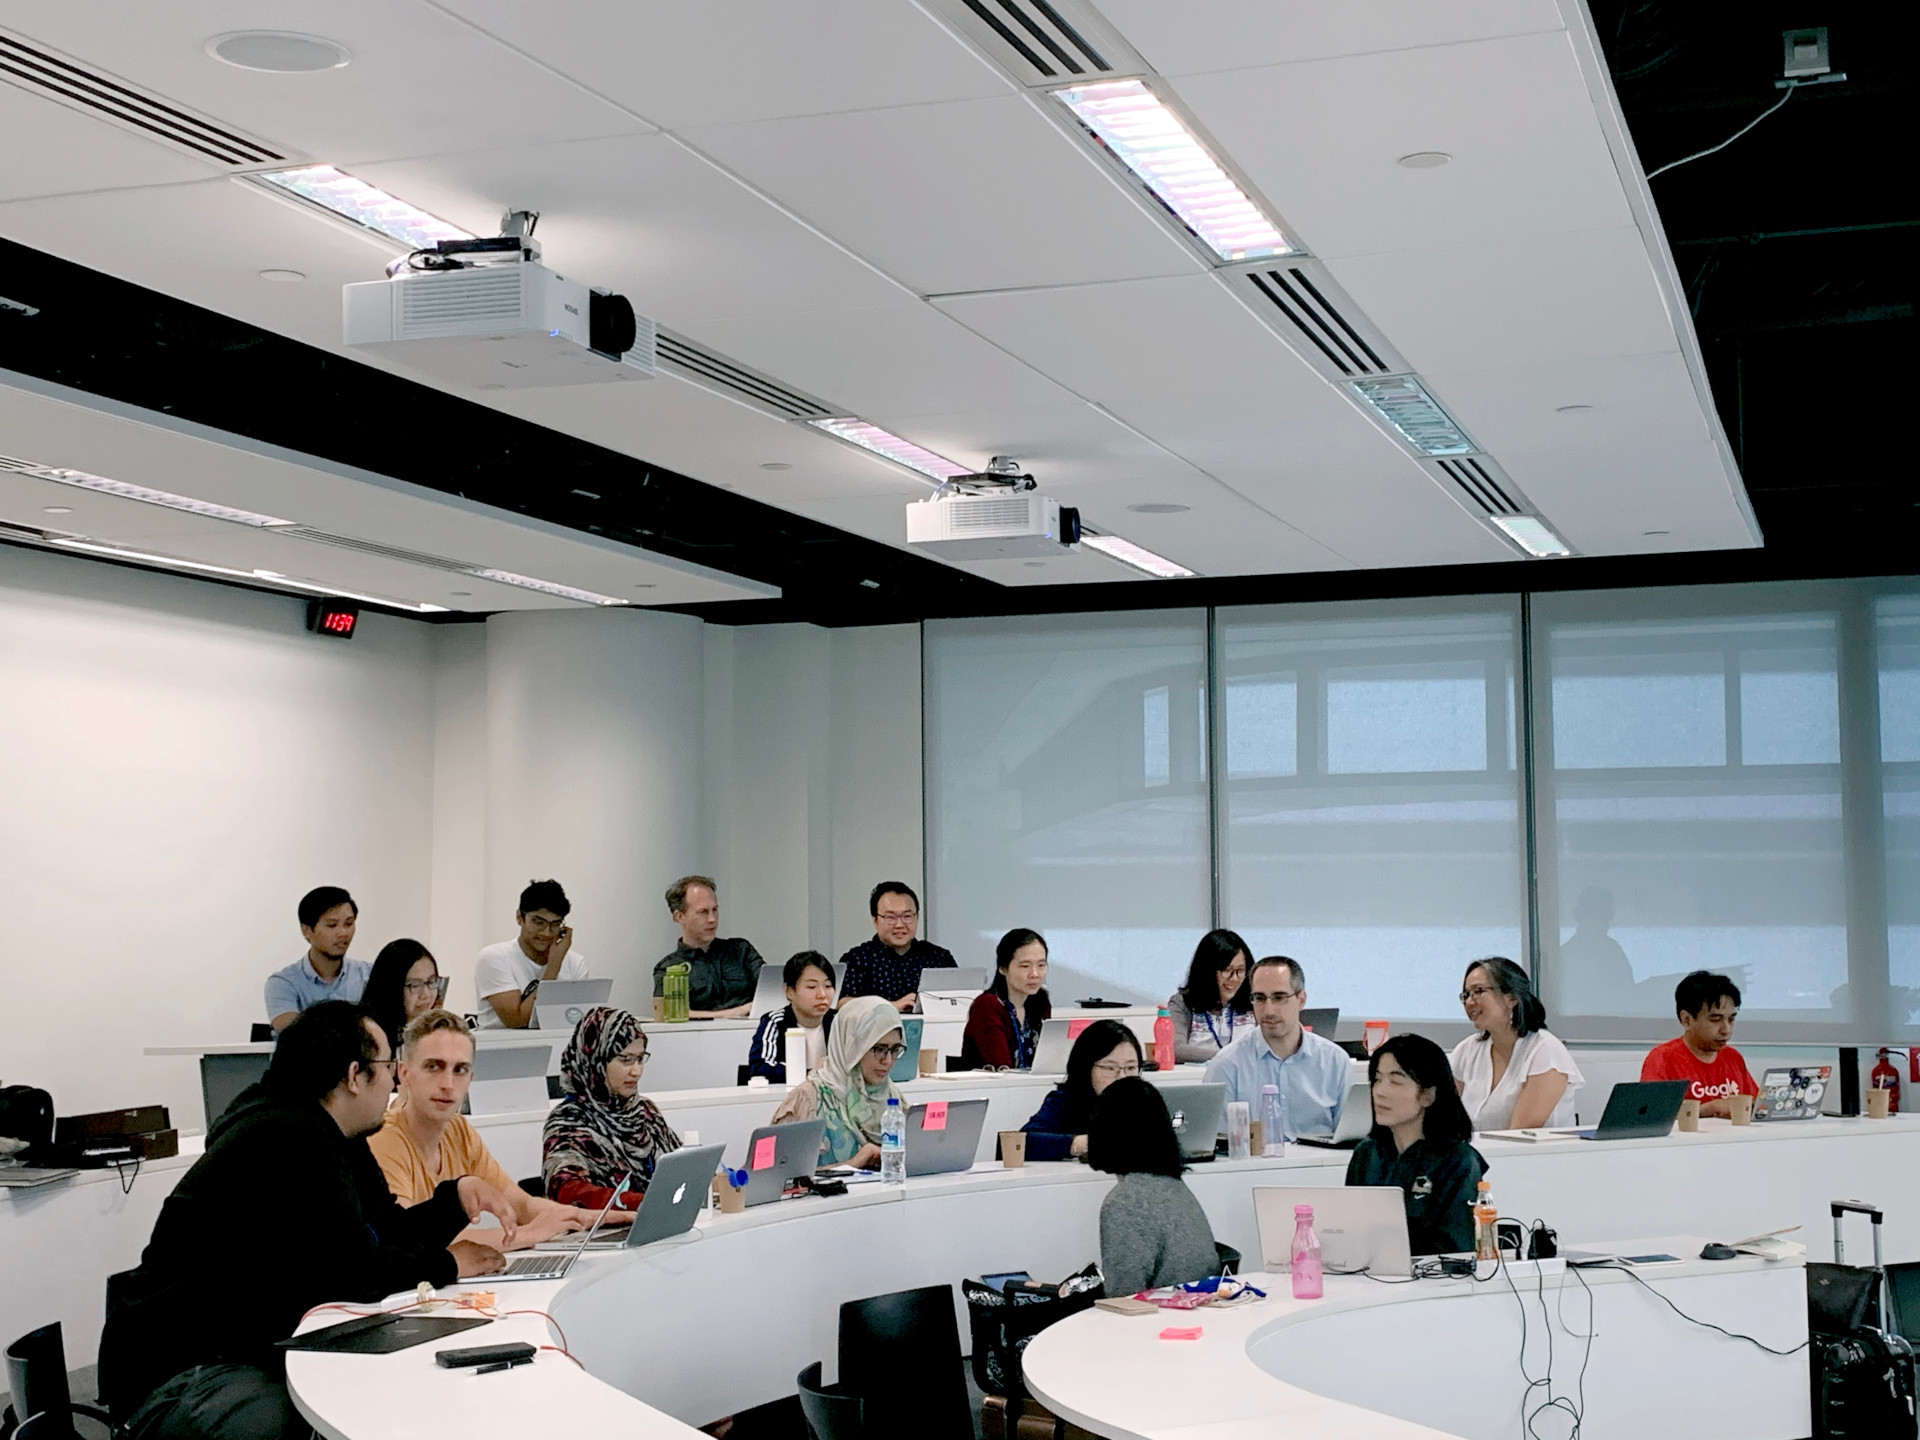
\includegraphics[width=0.75\linewidth]{assets/class}
\end{figure}
}
\only<3>{\centerline{to here\dots}
\begin{figure}
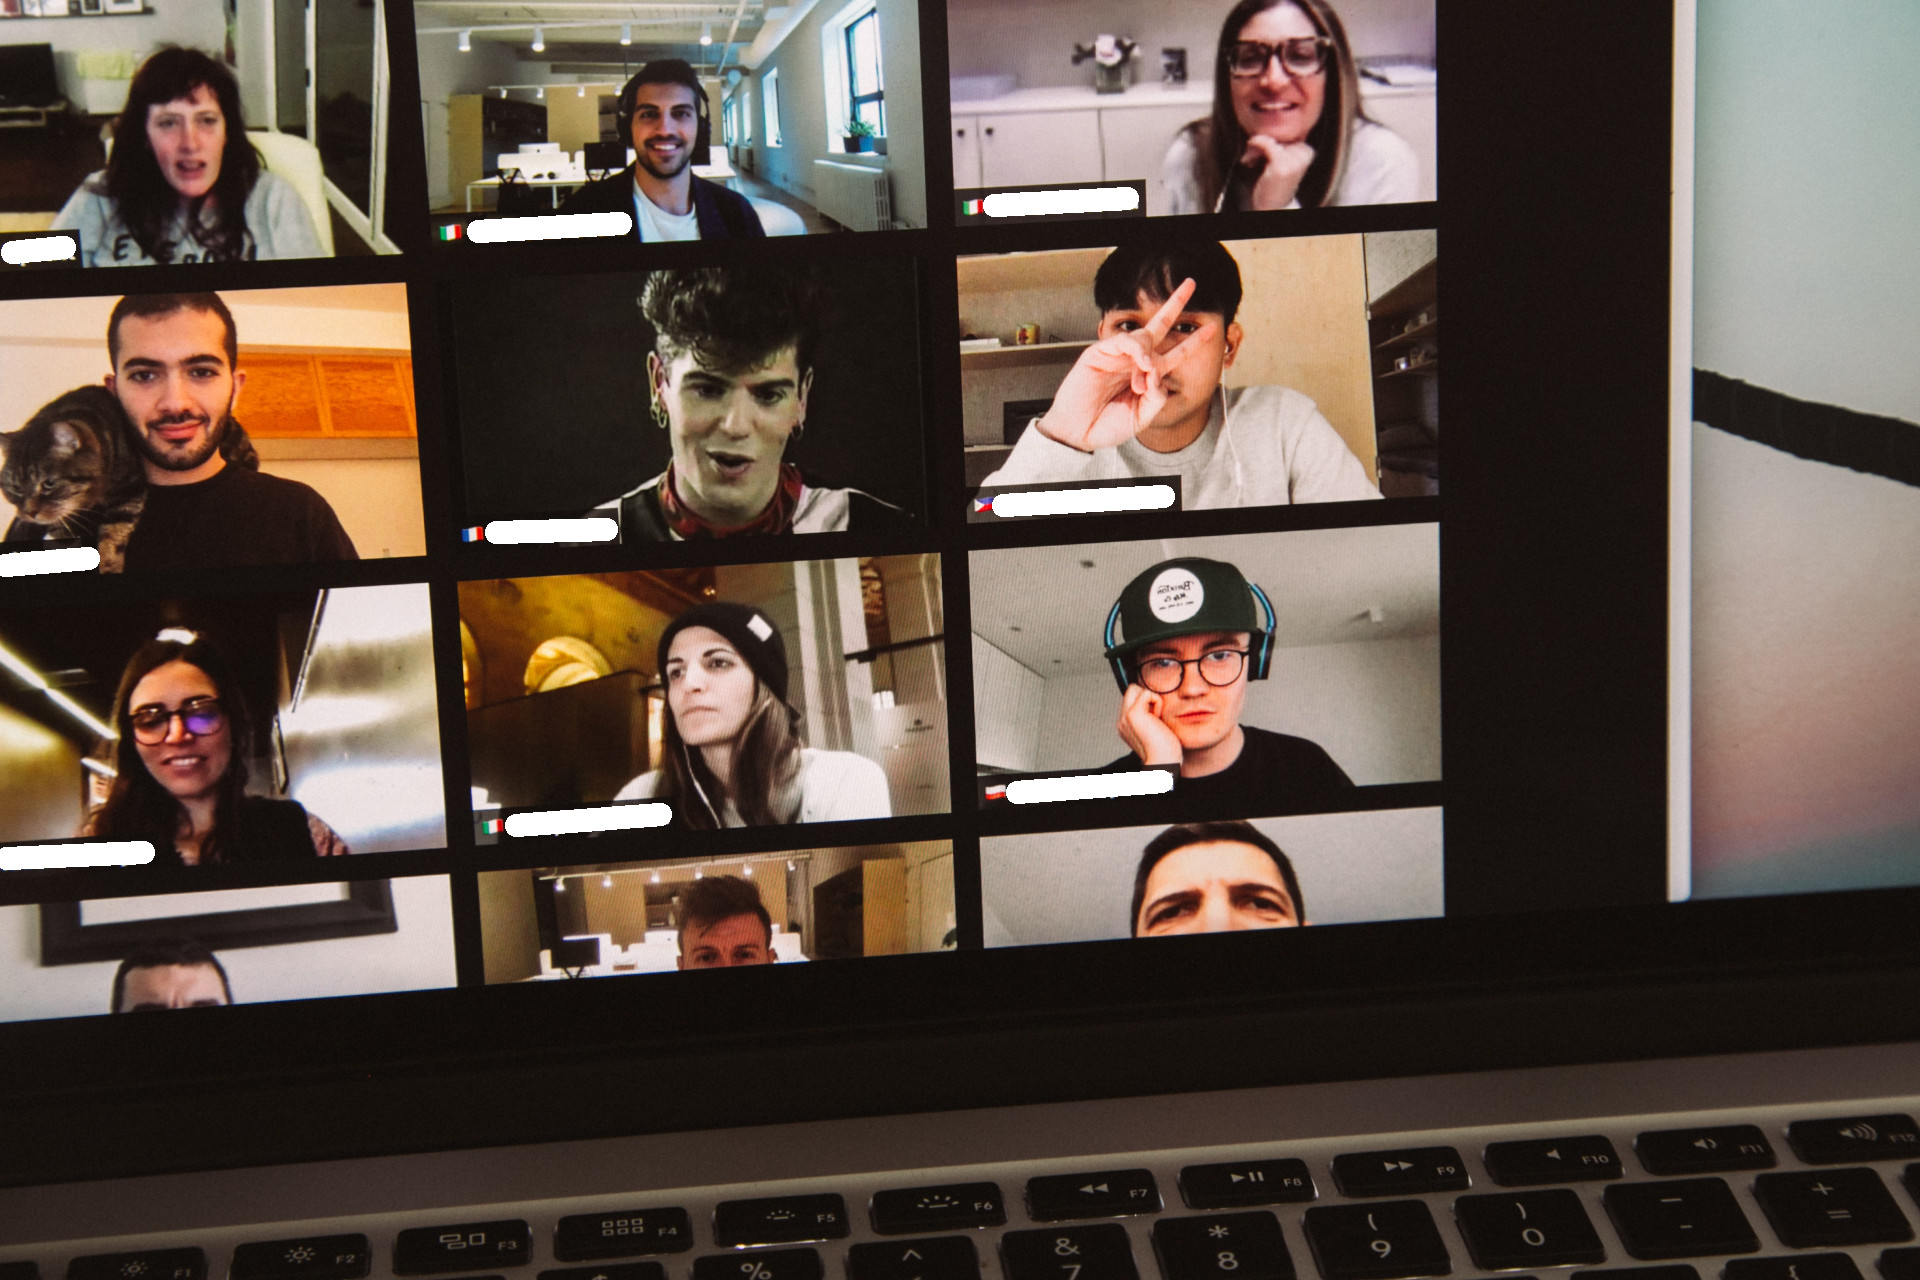
\includegraphics[width=0.85\linewidth]{assets/zoom}
\end{figure}
}
\only<4>{\centerline{without ending up here?}
\begin{figure}

\includegraphics[width=0.85\linewidth]{assets/zoom_fatigue}
\end{figure}
}
\end{frame}

\begin{frame}{Usefulness of Functional Programming}
\only<1>{
\centering\Large{\alert{3. Students question the usefulness of functional languages beyond academia}}}
\only<2>{
\begin{multicols}{2}

\begin{figure}

\includegraphics[width=0.8\linewidth]{assets/xkcd_haskell}
\caption*{\url{xkcd.com/1312}}
\end{figure}

\columnbreak

\begin{figure}

\includegraphics[width=0.8\linewidth]{assets/xkcd_tailrec}
\caption*{\url{xkcd.com/1270}}
\end{figure}
\end{multicols}
}
\end{frame}

%------------------------------------------------
\section{Course Structure and Conditions}
\begin{frame}{Hard Facts}
\begin{itemize}[<+->]
  \item 5 ECTS course (${\sim}150$ hours of work)
  \item 14 weeks; each week: one 90-minute lecture, one 90-minute tutorial, and one homework sheet
  \item Students took courses on Java, algorithms and data structures, discrete mathematics, and linear algebra.
   \item Winter semster 2019: 1057 students and 13 student assistants\\
   Winter semster 2020: 1031 students and 22 student assistants
\end{itemize}
\end{frame}

\begin{frame}{Syllabus}
We used Haskell, but most ideas apply to other functional languages.
\pause
\begin{itemize}[<+->]
  \item Basic FP concepts: recursion, pattern matching, list comprehension, polymorphism
  \item Formal proofs by structural and computation induction
  \item More FP concepts: higher-order functions, type classes, algebraic datatypes
  \item Specifics: modules, IO, lazy evaluation, tail recursion
\end{itemize}
\end{frame}



%------------------------------------------------
\begin{frame}[standout]
\Large{\alert{Any questions?}}

\end{frame}
%----------------------------------------------------------------------------------------
%\begin{frame}[allowframebreaks]{References}
  %\bibliography{../paper/sources.bib}
  %\bibliographystyle{abbrv}
%\end{frame}

% \begin{frame}[allowframebreaks]{Image Sources}
% \begin{itemize}
% \end{itemize}
% \end{frame}

\end{document}
